Optical flow \footnote{Optical flow,shorturl.at/mrtEZ}  คือรูปแบบของการเคลื่อนที่ของวัตถุในรูปภาพระหว่างภาพซึ่งอาจจะการจากเคลื่อน ที่ของวัตถุหรือตัวกล้อง ออกมาในรูปแบบของ เวกเตอร์(vector) 2 มิติ โดยที่เวกเตอร์แต่ละตัวจะแสดงถึงทิศทางการเคลื่อนที่ระหว่างภาพดังรูปด้านล่าง

\begin{figure}[!ht]
	\centering
	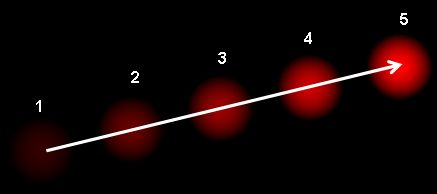
\includegraphics[width=1\textwidth]{chapter2/images/vector_optical.png}
		\caption{ตัวอย่างการเคลื่อนที่ของลูกบอล}
    	\label{fig:vector_optical}
\end{figure}

จากรูปภาพจะแสดงให้เห็นถึงการเคลื่อนที่ของลูกบอลของภาพที่ต่อเนื่องกัน 5 ภาพโดยที่ลูกศรแสดงถึงทิศทางการเคลื่อนที่ของเวกเตอร์
\\
\clearpage
\par
การทำงานของ optical flow อยู่บนสมมติฐานหลายประการได้แก่
\begin{enumerate}
	\setlength\itemsep{-0.25em}
	\item ความเข้มของพิกเซล(pixel) ของวัตถุจะไม่เปลี่ยนแปลงระหว่างภาพที่ต่อเนื่องกัน
	\item พิกเซลที่อยู่ใกล้กันจะมีการเคลื่อนไหวที่คล้ายกัน
\end{enumerate}

เมื่อพิจารณาพิกเซล I(x,y,t) จากภาพแรกจะเคลื่อนไหวเป็นระยะทาง (dx,dy) ไปยังภาพต่อไปหลังจากผ่านไปแล้ว dt เวลา ดังนั้นเนื่องจาก พิกเซล เหล่านี้เหมือนกันและความเข้มไม่มีการเปลี่ยนแปลง จึงทำให้พูดได้ว่า
\\
\centerline{$I(x,y,t) = I(x + dx, y + dy, t + dt)$}		\\
\centerline{$I$ คือ พิกเซลจากภายในภาพ}			\\
\centerline{$x$ คือ ตำแหน่งของพิกเซล ในแกน x} 		\\
\centerline{$dx$ คือ ระยะทางที่เคลื่อนที่ในแกน x} 		\\
\centerline{$y$ คือตำแหน่งของพิกเซลในแกน y} 		\\
\centerline{$dy$ คือ ระยะทางที่เคลื่อนที่ในแกน y}		\\
\centerline{$t$ คือ เวลา}						\\
\centerline{$dt$ คือ ระยะเวลาที่เปลี่ยนไประหว่างภาพ} 	\\

จากนั้นใช้การประมาณค่าของ taylor series ทางฝั่งขวามือและ ลบค่า common term และหารด้วย dt เพื่อให้ได้สมการดังต่อไปนี้
\\
\centerline{$f_{x}u + f_{y}v + f_{t} $}				\\
โดยที่
\\
\centerline{$f_{x} = \frac{\delta f}{\delta x} ; f_{y} = \frac{\delta f}{\delta y}$} 	\\
\centerline{$u = \frac{\delta x}{\delta t} ; v = \frac{\delta y}{\delta t}$}	 	\\
\centerline{$f_{x}$ คือ เกรเดียน(gradient) ในแกน x} 		\\
\centerline{$f_{y}$ คือ เกรเดียนในแกน y} 		\\
\centerline{$f_{y}$ คือ เกรเดียนของเวลา} 		\\
\centerline{$u$ คือ เวกเตอร์การเคลื่อนที่ของแกน x} 	\\
\centerline{$v$ คือ เวกเตอร์การเคลื่อนที่ของแกน y} 	\\

สมการข้างบนนี้จะเรียกว่าสมการ optical flow จากสมการทำให้สามารถหา $f_{x}$ และ $f_{y}$ โดยเป็น เกรเดียนของภาพ และ  $f_{t}$ เป็นเกรเดียน(gradient)ของเวลา แต่ $u$ กับ $v$ เป็นตัวแปรที่ไม่ทราบ ทำให้สมการนี้ไม่สามารถแก้ไขโดยมีตัวแปรที่ไม่ทราบถึง 2 ตัว จึงมีการนำวิธีการต่าง ๆ เข้ามาใช้ในการแก้ปัญหานี้ โดยวิธีการที่นำเข้ามาใช้ในการแก้ปัญหาคือ dense optical flow ซึ่งใช้อัลกอริทึมของ Gunner Farneback ซึ่งจะใช้วิธีการขยายพหุนาม\footnote{polynomial expansionfile:http://www.diva-portal.org/smash/get/diva2:273847/FULLTEXT01.pdf} (polynomial expansion)

